\subsection{Kiểm Định Hình Thức}

\subsubsection{Kiểm Định Durbin--Watson}

Kiểm định Durbin--Watson dùng để phát hiện tự tương quan bậc 1 trong phần dư của mô hình hồi quy. Giả thuyết thường viết là:
\[
  H_0:\rho=0 \quad \text{(không có tự tương quan bậc 1)},
\]
\[
  H_1:\rho\neq 0,
  \qquad \text{hoặc} \qquad
  H_1:\rho>0,
  \qquad \text{hoặc} \qquad
  H_1:\rho<0.
\]
Thống kê Durbin--Watson là:
\[
  d = \frac{\sum_{t=2}^{n}(e_t-e_{t-1})^2}{\sum_{t=1}^{n}e_t^2}.
\]
Giá trị $d$ nằm trong khoảng $0\le d\le 4$ và có quan hệ gần đúng:
\[
  d\approx 2(1-\hat{\rho}).
\]
Do đó, $d\approx 2$ gợi ý chưa có tự tương quan bậc 1 rõ ràng; $d<2$ gợi ý tự tương quan dương; $d>2$ gợi ý tự tương quan âm.

\subsubsection{Cách Đọc Bảng Durbin--Watson}

Để kết luận theo bảng, so sánh $d$ với hai giá trị tới hạn $d_L$ và $d_U$, phụ thuộc vào số quan sát $n$, số biến độc lập $k$ và mức ý nghĩa $\alpha$.

\begin{figure}[H]
  \centering
  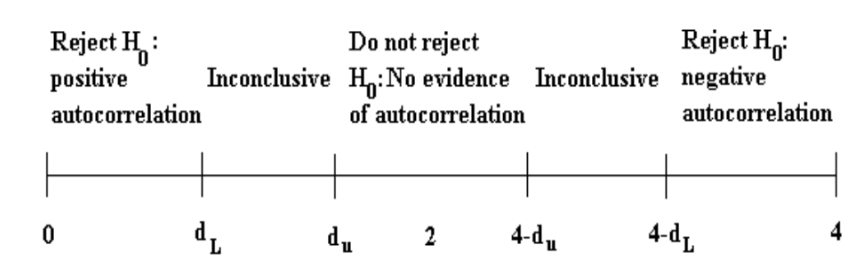
\includegraphics[width=0.9\textwidth]{./media/image2.png}
  \caption{Vùng quyết định của kiểm định Durbin--Watson. Vùng giữa $d_U$ và $4-d_U$ là vùng chưa có bằng chứng tự tương quan; hai vùng gần $0$ và $4$ lần lượt nghiêng về tự tương quan dương và âm.}
  \label{fig:durbin_watson_regions}
\end{figure}

Quy tắc đọc:
\begin{itemize}
  \item Nếu $0<d<d_L$: bác bỏ $H_0$, kết luận có tự tương quan dương.
  \item Nếu $d_L\le d\le d_U$: vùng không kết luận được.
  \item Nếu $d_U<d<4-d_U$: không bác bỏ $H_0$.
  \item Nếu $4-d_U\le d\le 4-d_L$: vùng không kết luận được.
  \item Nếu $4-d_L<d<4$: bác bỏ $H_0$, kết luận có tự tương quan âm.
\end{itemize}

Khi dùng R, hàm \texttt{dwtest()} trong gói \texttt{lmtest} cung cấp trực tiếp thống kê $d$ và p-value, nên có thể kết luận theo p-value.

\subsubsection{Hạn Chế Của Durbin--Watson}

Durbin--Watson chủ yếu phù hợp với tự tương quan bậc 1. Nếu nghi ngờ tự tương quan bậc cao hơn hoặc mô hình có biến phụ thuộc trễ ở vế phải, Durbin--Watson không còn là lựa chọn tốt nhất. Khi đó, kiểm định Breusch--Godfrey tổng quát hơn.

\subsubsection{Kiểm Định Breusch--Godfrey}

Breusch--Godfrey kiểm tra tự tương quan đến bậc $p$. Giả sử sai số có thể phụ thuộc vào các độ trễ:
\[
  \varepsilon_t
  =
  \rho_1\varepsilon_{t-1}
  + \rho_2\varepsilon_{t-2}
  + \cdots
  + \rho_p\varepsilon_{t-p}
  + v_t.
\]
Giả thuyết kiểm định:
\[
  H_0:\rho_1=\rho_2=\cdots=\rho_p=0,
\]
\[
  H_1:\text{ có ít nhất một }\rho_j\neq 0.
\]

Vì không quan sát được $\varepsilon_t$, ta dùng phần dư $e_t$ từ mô hình gốc và chạy hồi quy phụ:
\[
  e_t
  =
  \alpha_0
  + \alpha_1X_{1t}
  + \cdots
  + \alpha_kX_{kt}
  + \rho_1e_{t-1}
  + \cdots
  + \rho_pe_{t-p}
  + v_t.
\]
Sau đó tính:
\[
  LM = nR^2_{aux} \sim \chi^2(p)
\]
dưới $H_0$ với mẫu đủ lớn. Bác bỏ $H_0$ khi p-value nhỏ hơn $\alpha$.

\textbf{Chọn bậc $p$.} Không nên chọn $p$ tùy ý. Với dữ liệu tháng, $p=12$ có thể dùng để kiểm tra phụ thuộc mùa vụ cùng tháng năm trước; với dữ liệu quý, $p=4$ thường là mốc cần cân nhắc.

% -----------------------------------------------------------------------------
